\documentclass{article}
\usepackage[preprint]{neurips_2026}
\usepackage[T1]{fontenc}
\usepackage{amsmath,amssymb,booktabs,graphicx,microtype}
\usepackage{hyperref}
\usepackage{xcolor}
\usepackage{url}

% This is an NUS course report, not a NeurIPS preprint; retain the template's
% preprint layout while suppressing only its first-page notice text.
\makeatletter
\renewcommand{\@noticestring}{}
\makeatother

\title{Difficulty Matters: A Controlled Study of Difficulty Metrics for
Curriculum Behavior Cloning in Robotic Manipulation}

\author{Xiaoda Zhong\\
  \textit{National University of Singapore}\\
  \url{https://github.com/Xiaoda-Zhong/cs5478-difficulty-curriculum-bc}}

\begin{document}
\maketitle

\begin{abstract}
Behavior cloning (BC) learns manipulation from demonstrations, yet small
prediction errors can compound during closed-loop execution. Difficulty-based
curricula may help by staging which demonstrations are sampled, but Task,
Expert, and Learner notions of difficulty need not agree. We compare these
three scores and five schedules under matched
architectures, initializations, and optimizer-update budgets on simulated
Franka Panda manipulation. In pick-and-place, Task and Expert scores correlate
strongly, while Learner error induces a substantially different ranking. None
of the three easy-to-hard schedules consistently improves over uniform
sampling. Reverse Learner has the highest observed mean Fresh-ID success
(81.5\% versus 69.3\% for Uniform), but its advantage is seed-sensitive and
its development learning AUC is nearly identical to Uniform; this is not
evidence of statistically established superiority. In an exploratory
object-stacking evaluation, all methods achieve low success rates, with no
curriculum outperforming uniform sampling. The results show that curriculum
conclusions depend on both the difficulty definition and the staged exposure
schedule, and require closed-loop evaluation.
\end{abstract}

\section{Introduction}
\label{sec:introduction}

Behavior cloning (BC) turns robot learning into supervised learning from
expert state--action pairs. Its simplicity is attractive for manipulation,
where online exploration can be unsafe or expensive. Yet a policy trained on
expert states is evaluated on states induced by its own actions. Small errors
can therefore compound and move the robot outside the demonstration
distribution, a classical limitation of offline imitation
\citep{pomerleau1989alvinn,ross2011dagger}. How demonstrations are sampled
during optimization may influence both learning speed and the final policy.

Curriculum learning proposes to organize examples rather than sample them
uniformly \citep{bengio2009curriculum}. In manipulation, however, ``easy'' is
ambiguous. A task can be geometrically demanding; an expert can require a long
or circuitous execution; or a learner can predict a demonstration poorly.
These notions need not agree. Moreover, easy-to-hard is not the only plausible
direction: difficult examples can expose useful decision boundaries early,
motivating a reverse ordering related to hard-example and reverse-curriculum
ideas \citep{florensa2017reverse}.

We study three questions: \textbf{RQ1 (ranking agreement):} do Task-, Expert-,
and Learner-based scores produce consistent trajectory rankings?
\textbf{RQ2 (failure prediction):} do these scores predict closed-loop BC
failures? \textbf{RQ3 (curriculum effectiveness):} under matched training
budgets and initialization protocols, how do staged curricula based on these
scores compare with uniform sampling? The stages change cumulative exposure as
well as order, so RQ3 concerns demonstration-pool sampling schedules rather
than pure permutations with equal exposure.

We construct all scores on one frozen split, evaluate five schedules, analyze
failure prediction and ranking corruption, and repeat the comparison on
stacking as an exploratory secondary evaluation. We propose no new curriculum
algorithm; the contribution is a controlled empirical analysis.

The results are mixed in an informative way. On pick-and-place, task and
expert difficulty correlate at $0.842$, while learner difficulty correlates
negatively with each. Learner difficulty has the largest point-estimate
failure AUROC, but its confidence interval includes chance. Reverse Learner
has the highest observed pick-and-place Fresh-ID mean, although its seed-level
advantage is inconsistent. Stacking is near the performance floor, where no
curriculum outperforms Uniform. Thus the evidence cautions against treating
either difficulty definitions or schedule effects as task-independent.

\section{Related Work}
\label{sec:related}

\paragraph{Imitation learning and robotic demonstrations.}
Behavior cloning directly regresses expert actions and has a long history in
autonomous control \citep{pomerleau1989alvinn}. Surveys of learning from
demonstration emphasize the importance of representation, demonstration
quality, and correspondence between teacher and learner
\citep{argall2009survey,osa2018survey}. Offline BC avoids environment
interaction during training but suffers covariate shift. DAgger addresses this
by collecting expert labels on learner-induced states
\citep{ross2011dagger}; our study deliberately retains a fixed offline dataset
without interactive data collection. Offline manipulation studies show
sensitivity to demonstration quality, algorithm design, and stopping criteria
\citep{mandlekar2022what}; data-quality work formalizes curation through
distribution shift \citep{belkhale2023data}. We instead vary staged sampling
over one fixed scripted-expert dataset.

\paragraph{Curriculum learning for sequential decision-making.}
Curriculum learning orders training examples from easier to harder and can
improve optimization or generalization in some settings
\citep{bengio2009curriculum}. Automated curriculum research broadens this
view to task selection and teacher--student formulations
\citep{portelas2020survey}. Reverse curriculum generation has also shown that
starting near successful states and expanding outward can aid sparse-reward
control \citep{florensa2017reverse}. Our Reverse Learner condition is more
limited: it reverses a fixed demonstration ranking and does not generate new
tasks or states. Cross-Episodic Curriculum (CEC) instead structures sequences
of online learning trials and mixed-quality demonstrations within a
Transformer's context to improve agent learning across episodes
\citep{shi2023cross}. Recent preprint work, CurriBuffer, applies
difficulty-aware demonstration selection, curriculum sampling, and retrieval
to Vision-Language-Action policy specialization
\citep{hosseini2026curribuffer}. These approaches establish the
relevance of organizing experience for sequential and robotic policies. Our
setting is deliberately narrower: it uses fixed offline BC data and compares
difficulty definitions without cross-episodic context or retrieval.
Classification studies further show that scoring and pacing are distinct
design choices \citep{hacohen2019power}, and that curriculum,
anti-curriculum, and random schedules depend on training budget and data noise
\citep{wu2021when}.

\paragraph{Difficulty estimation and curriculum design.}
Example difficulty may be based on task metadata, teacher effort, uncertainty,
loss, or forgetting. These signals describe different phenomena, and
loss-based signals risk in-sample bias. Rampp et al. systematically study the
similarity and robustness of difficulty scoring functions and their effects on
curriculum learning in image and acoustic-scene classification
\citep{rampp2024difficulty}. We extend this question to trajectory-level BC and
closed-loop robotic manipulation. Specifically, we compare Task difficulty
(initial geometry), Expert difficulty (demonstration effort), and Learner
difficulty (five-fold out-of-fold prediction error). These are descriptive
signals rather than ground-truth measures of complexity.

Taken together, CEC and CurriBuffer motivate curriculum organization for
sequential and robotic learning, while Rampp et al. motivate comparing how
difficulty is defined. We hold the demonstrations, policy family, and training
budget fixed while comparing three trajectory rankings and five staged
sampling schedules under physical closed-loop evaluation.

\section{Method}
\label{sec:method}

\subsection{Problem formulation and behavior cloning}
A demonstration $\tau_i=\{(s_{it},a_{it})\}_{t=1}^{T_i}$ contains observed
robot/task state $s$ and expert action $a=(a^{\mathrm{mot}},a^{\mathrm{grip}})$.
The motion component is a three-dimensional Cartesian displacement; the
gripper component is binary. A shared MLP produces a motion vector and one
gripper logit. With training-only observation statistics $\mu,\sigma$ and
motion scale $s_a$, we optimize
\begin{equation}
\mathcal{L}=
\left\|\hat a^{\mathrm{mot}}/s_a-a^{\mathrm{mot}}/s_a\right\|_2^2
+\operatorname{BCE}(\hat a^{\mathrm{grip}},a^{\mathrm{grip}}).
\end{equation}
At inference, motion is rescaled and norm-clipped to the largest training
expert step. Evaluation is autonomous and closed loop; expert actions are
never used during policy rollouts.

\subsection{Difficulty definitions}
All scores are trajectory-level and use only the 240 training trajectories.
For a component $x$, $z(x)=(x-\mu_x)/(\sigma_x+\epsilon)$ uses statistics from
that split.

\paragraph{Task difficulty.}
For pick-and-place, the components are initial end-effector--object distance,
object--goal distance, and inverse target radius $1/r$:
\begin{equation}
d_{\mathrm{task}}(\tau)=\tfrac13[z(d_{\mathrm{EE,obj}})
+z(d_{\mathrm{obj,goal}})+z(1/r)].
\end{equation}
They represent approach distance, transport distance, and placement precision.

\paragraph{Expert difficulty.}
We average standardized duration $T$, executed end-effector path length $L$,
and cumulative Cartesian action magnitude $A$:
\begin{equation}
d_{\mathrm{expert}}(\tau)=\tfrac13[z(T)+z(L)+z(A)].
\end{equation}
These strongly correlated components measure execution effort; $L$ and $A$
are especially redundant in our deterministic controller.

\paragraph{Learner difficulty.}
We partition the training trajectories into five folds. For each fold, a new
BC model with the same $128$--$128$ architecture trains for 95 fixed epochs on
192 trajectories with fold-only normalization and motion scaling, then scores
the unseen 48. This differs from the 20,600-update curriculum budget. Every
trajectory is scored exactly once:
\begin{equation}
d_{\mathrm{learner}}(\tau)=\frac{1}{T}\sum_{t=1}^{T}
\left\|\frac{\hat a_t^{\mathrm{mot}}-a_t^{\mathrm{mot}}}{s_a}\right\|_2^2.
\end{equation}
Gripper BCE is retained as a diagnostic but excluded from the primary score.
Out-of-fold scoring avoids assigning low difficulty merely because a model
memorized a training trajectory; it measures approximation error for this
policy family, not intrinsic task complexity or failure probability.

\subsection{Curriculum strategies}
Each metric sorts trajectories by ascending score, breaking ties by ID, and
forms 80 Easy, 80 Medium, and 80 Hard trajectories. Forward curricula use
Easy, then Easy+Medium, then all data. Reverse Learner uses Hard, then
Hard+Medium, then all data. Uniform uses all trajectories throughout.
Curriculum boundaries are updates 6,866 and 13,733 of a 20,600-update run.
Within a seed, all methods share the exact initial weights, architecture,
optimizer settings, loss, validation split, and evaluation tasks; only the
eligible trajectory pool differs.

Sampling is uniform over \emph{transitions} in the eligible pool, not uniform
over trajectories. Thus longer trajectories receive more aggregate sampling
probability. The three stages contain 6,866, 6,867, and 6,867 updates. Using
the actual transition counts, cumulative expected group exposures are
59.9/28.1/12.0\% (Task), 59.5/28.3/12.1\% (Expert), and
61.9/27.6/10.6\% (Learner) for Easy/Medium/Hard. Reverse Learner yields
11.6/28.3/60.1\% in that order. Uniform exposure follows each ranking's
transition composition (Task: 31.2/32.9/36.0\%; Expert: 30.6/33.1/36.3\%;
Learner: 34.7/33.6/31.7\%). Consequently, the methods compare staged
pool-sampling schedules that combine ordering with cumulative reweighting; they
do not isolate order under equal per-trajectory exposure.

\section{Experiments and Results}
\label{sec:experiments}

\subsection{Experimental setup}
The primary task is PyBullet pick-and-place with a Franka Panda. The 10D state
contains end-effector, cube, and goal positions (three coordinates each) plus
mean finger opening. The action is a 3D Cartesian delta and binary gripper
command. Target radius affects success and Task difficulty but is not observed
by the policy.
A deterministic finite-state expert physically grasps, transports, releases,
and retreats. We collect 300 successful demonstrations (65,738 transitions)
and freeze a trajectory-level 240/60 train/validation split. Policies use a
$10\!\rightarrow\!128\!\rightarrow\!128$ ReLU MLP with separate motion and
gripper heads. AdamW uses learning rate $10^{-3}$ and batch size 256. Each
curriculum has 20,600 updates and seeds 5478, 5479, and 5480. Evaluation tasks
and difficulty groups are frozen before policy comparison. An episode succeeds
when cube--goal horizontal distance is below the sampled radius and vertical
error is below 0.025~m; the horizon is 400 actions.

The demonstrations are generated by a closed-loop finite-state controller,
not by teleporting the cube or constraining it to the gripper. Each trajectory
includes physical approach, finger closure, lift, transport, placement,
release, and retreat. Cube and goal $x$ positions vary in $[0.42,0.63]$~m;
their $y$ ranges are $[-0.28,0.12]$ and $[-0.12,0.28]$~m, with at least
0.18~m separation. Target radii vary in $[0.045,0.075]$~m, while robot
initialization and simulator settings remain fixed. Dataset and
evaluation-task fingerprints prevent accidental regeneration or overlap.
Complete trajectories, rather than individual transitions, are assigned to
training and validation sets.

Figure~\ref{fig:pnp-simulation-sequence} shows one deterministic successful
expert rollout rendered directly by the PyBullet camera. The four frames come
from the same trajectory and show the physical finger grasp, lifted transport,
and release over the goal marker.

\begin{figure*}[t]
  \centering
  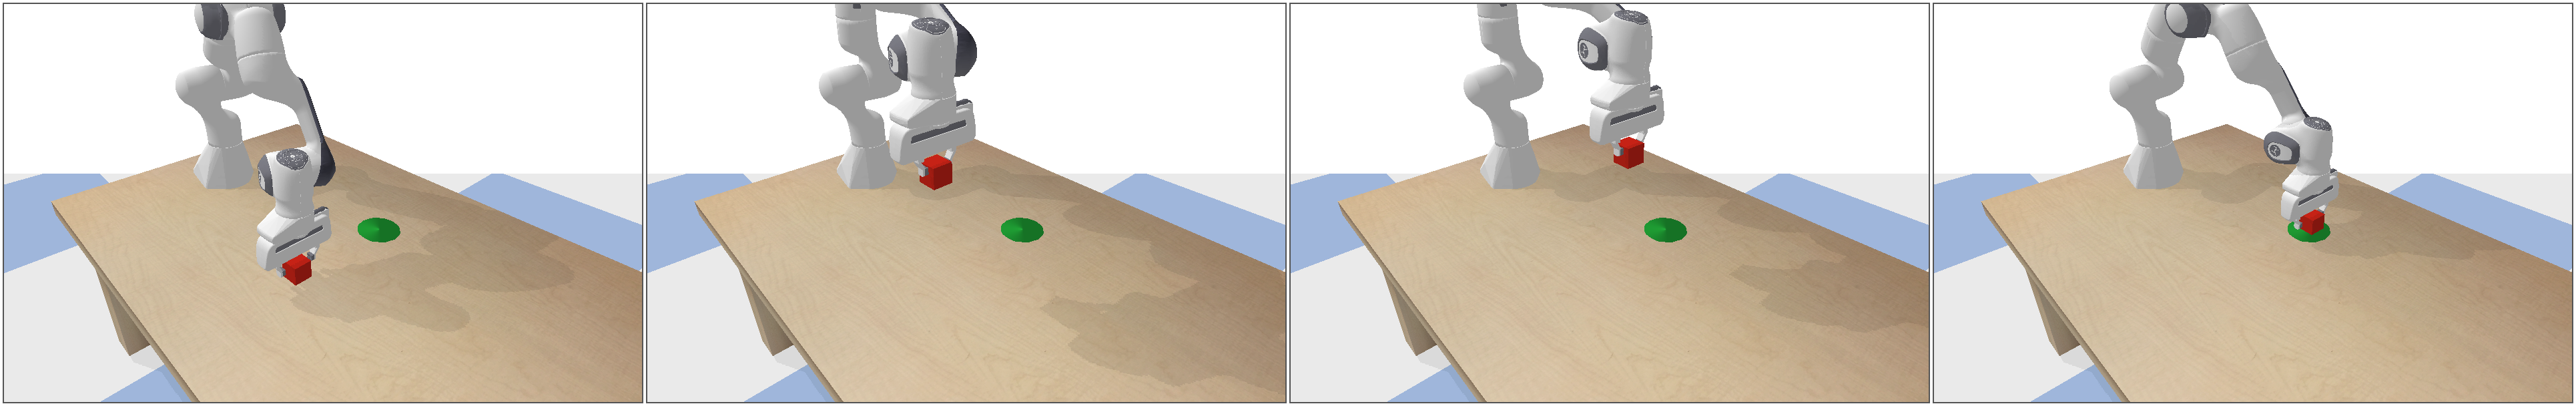
\includegraphics[width=\textwidth]{figures/pnp_simulation_sequence.png}
  \caption{Real PyBullet states from one successful deterministic
  pick-and-place expert rollout: (a) final pre-grasp approach, (b) grasped
  cube after lift, (c) mid-transport, and (d) placement and gripper release.
  The robot advances only through the environment action interface; the cube
  is neither teleported nor attached by an artificial constraint.}
  \label{fig:pnp-simulation-sequence}
\end{figure*}

An initial unscaled policy reaches 0/100 closed-loop success despite high
offline gripper accuracy. Scaling Cartesian targets by the maximum expert step
($0.008$~m) reduces validation motion error and raises a separately developed
Uniform baseline to 83/100. All controlled curriculum runs use this scaled
formulation from scratch; the historical 83/100 checkpoint is not substituted
for matched Uniform. This prevents a development-selected checkpoint from
receiving an unfair advantage in the controlled comparison.

The 60-trajectory validation split supplies offline loss only. Closed-loop
learning curves use a separate frozen 100-task development set. Final reporting
uses 200 new Fresh-ID tasks and two disjoint 100-task OOD sets; none selects a
checkpoint.

\subsection{Difficulty metrics and failure prediction}
\label{sec:difficulty-results}
The metrics disagree substantially (Figure~\ref{fig:pnp-corr}). Spearman
correlations are $0.842$ (Task--Expert), $-0.453$ (Task--Learner), and $-0.543$
(Expert--Learner). Geometry and scripted execution effort therefore align,
whereas trajectories predicted poorly by held-out learners tend not to be the
same ones ranked hard by those measures.

\begin{figure}[t]
  \centering
  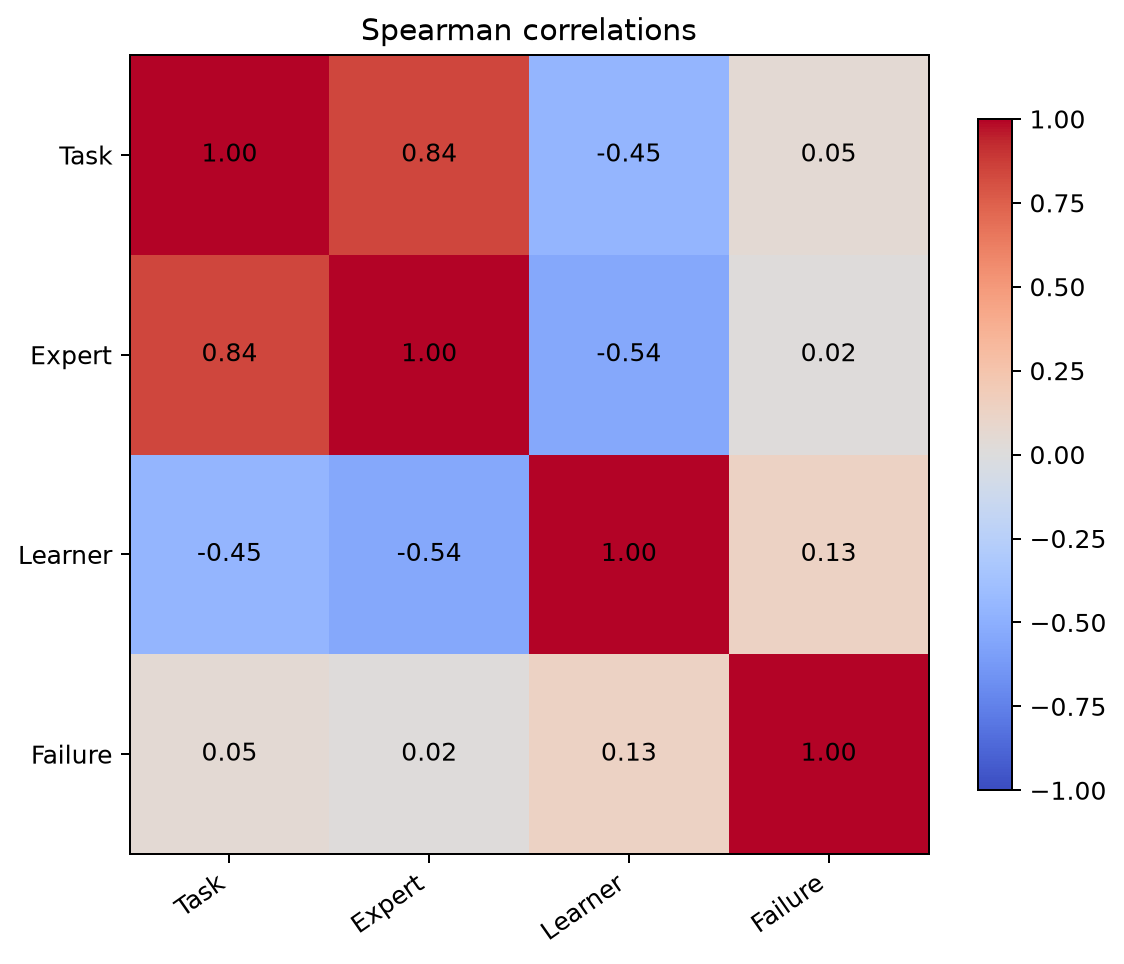
\includegraphics[width=.58\linewidth]{figures/pnp_difficulty_correlation.png}
  \caption{Spearman correlations among Task, Expert, and Learner scores and
  binary out-of-fold rollout failure. The weak score--failure correlations
  complement the AUROC analysis; Learner difficulty disagrees with geometry
  and expert effort.}
  \label{fig:pnp-corr}
\end{figure}

We next reconstruct each demonstrated task and run its out-of-fold policy.
The policies solve 198/240 tasks. Failure AUROC is $0.540$ for Task
($95\%$ bootstrap CI $[0.441,0.647]$), $0.512$ for Expert
($[0.423,0.607]$), and $0.598$ for Learner ($[0.494,0.692]$). Learner has the
largest point estimate, but every interval includes 0.5 and paired-difference
intervals include zero; this does not establish a statistically reliable
winner. Intervals use 1,000 stratified trajectory-level bootstrap resamples.

The Easy/Medium/Hard outcomes also resist a simple interpretation. Task-score
failure rates are 17.5\%, 13.7\%, and 21.3\%; Expert-score rates are 16.2\%,
21.3\%, and 15.0\%; Learner-score rates are 13.7\%, 16.2\%, and 22.5\%.
Only the learner ordering exhibits the intended monotonic increase, and even
there the sample is modest. Grasp and release have the largest expert-phase
prediction errors, while learner-error outliers are unevenly distributed
across OOF folds. A continuous association therefore need not create clean
behavioral regimes after a three-way split.

\subsection{Controlled curriculum learning}
Table~\ref{tab:m7} reports the predefined final checkpoint and normalized
learning-curve AUC. ``Hard'' denotes the 34 hardest of the 100 frozen
development tasks under the Task score using frozen training normalization.
Reverse Learner has the highest observed final and hard-case success, but only
three seeds are available and variance is large.
Its AUC is effectively tied with Uniform, so higher final success should not be
interpreted as clearly faster convergence. Figure~\ref{fig:pnp-curves} shows
the seed-averaged trajectories.

Seed-level outcomes reveal why averages require care. Uniform obtains 80\%,
47\%, and 100\% development success; Task obtains 24\%, 62\%, and 86\%; Expert
obtains 61\%, 61\%, and 37\%; Learner obtains 88\%, 41\%, and 65\%; and Reverse
Learner obtains 84\%, 72\%, and 98\%. Initial weights are matched across
methods within a seed but intentionally differ across seeds. The high spread
is therefore part of the training outcome rather than evaluation-task noise.
Offline validation losses cluster narrowly between 0.00591 and 0.00661 and do
not reproduce the rollout ordering, further motivating closed-loop evaluation.

\begin{table}[t]
\centering
\caption{Pick-and-place development results on 100 frozen tasks, mean $\pm$
sample SD over three seeds. Hard success uses the 34 Task-Hard tasks. Bold
marks only the largest observed mean, not statistical significance.}
\label{tab:m7}
\small
\begin{tabular}{lccc}
\toprule
Method & Final success & Learning AUC & Hard success \\
\midrule
Uniform & $75.7\!\pm\!26.8$ & $0.784\!\pm\!0.054$ & $66.7\!\pm\!32.4$ \\
Task & $57.3\!\pm\!31.3$ & $0.588\!\pm\!0.203$ & $51.0\!\pm\!35.1$ \\
Expert & $53.0\!\pm\!13.9$ & $0.611\!\pm\!0.099$ & $52.0\!\pm\!17.2$ \\
Learner & $64.7\!\pm\!23.5$ & $0.604\!\pm\!0.136$ & $62.7\!\pm\!23.8$ \\
Reverse Learner & $\mathbf{84.7\!\pm\!13.0}$ & $0.787\!\pm\!0.003$ & $\mathbf{91.2\!\pm\!7.8}$ \\
\bottomrule
\end{tabular}
\end{table}

Difficulty-stratified Fresh-ID performance provides a complementary view.
Uniform achieves 74.1\%, 72.6\%, and 61.1\% on Task-defined Easy, Medium, and
Hard groups. Reverse Learner achieves 82.6\%, 78.6\%, and 83.3\%. Groups are
fixed using training-set task-score normalization before observing outcomes.
They represent task-defined strata, not calibrated probabilities of failure.
Likewise, paired comparisons over 200 tasks describe task-level differences
but do not replace independent training seeds.

\begin{figure}[t]
  \centering
  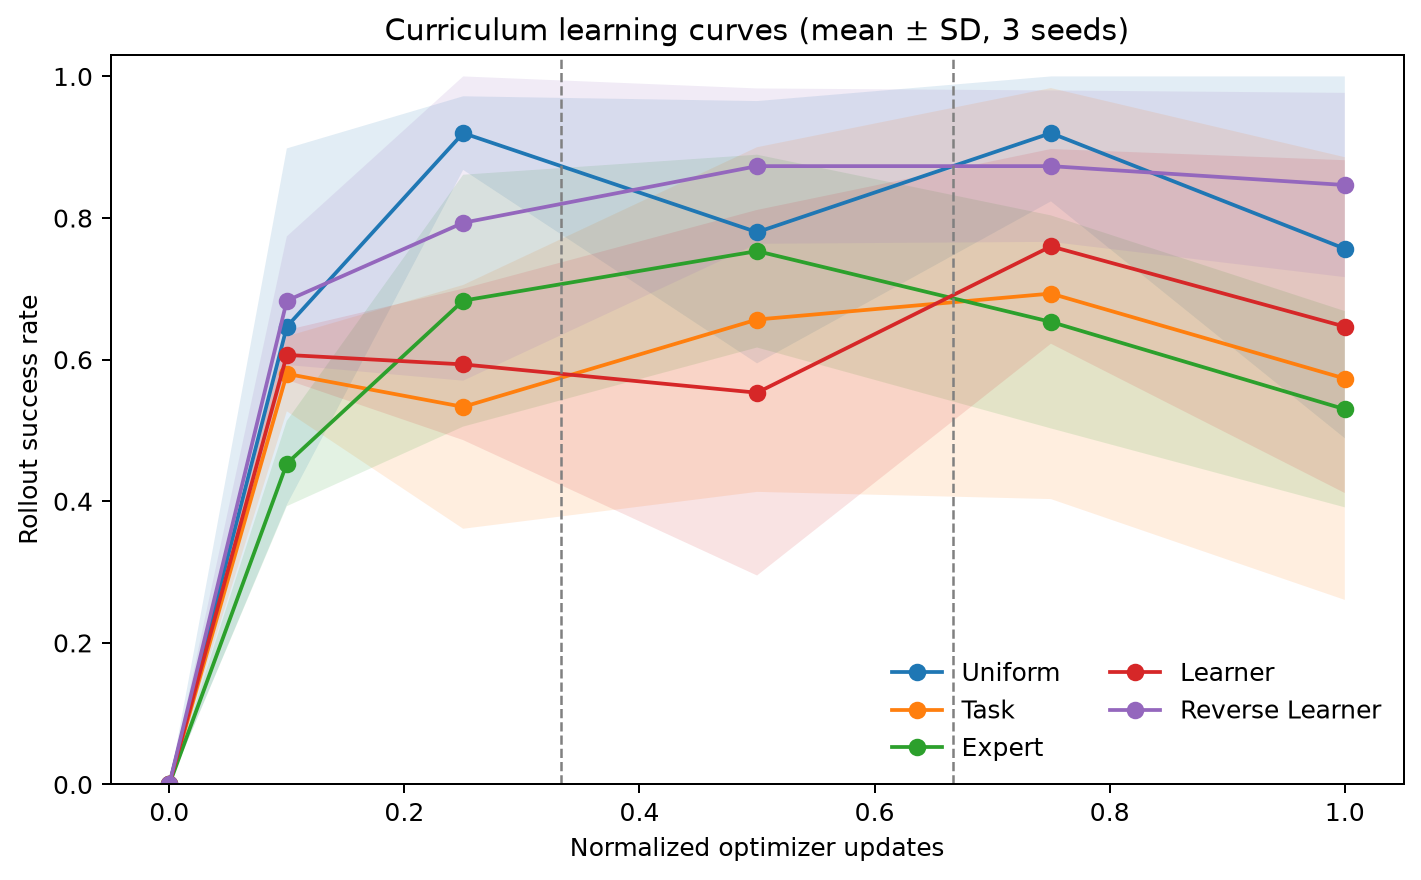
\includegraphics[width=.72\linewidth]{figures/pnp_learning_curves.png}
  \caption{Pick-and-place closed-loop learning curves (mean $\pm$ sample SD)
  on 100 frozen development tasks. Evaluations occur at initialization and at
  10, 25, 50, 75, and 100\% of updates; dashed lines mark stage boundaries.
  AUC integrates success over normalized progress, including update zero.
  Curves do not select the final model.}
  \label{fig:pnp-curves}
\end{figure}

\subsection{Fresh-ID and out-of-distribution evaluation}
\label{sec:final-eval}
Table~\ref{tab:m8} evaluates the final 20,600-update checkpoint on 200 frozen
Fresh-ID tasks, 100 Precision-OOD tasks with unchanged spatial ranges but
radius $[0.030,0.044]$~m, and 100 Spatial-OOD tasks with cube $x$ shifted to
$[0.390,0.415]$~m while other ranges remain standard.
Reverse Learner has the highest mean on all three splits, followed by Uniform
on Fresh-ID. Nevertheless, several OOD means exceed their ID counterpart, so
OOD should not be equated automatically with greater empirical difficulty.
Precision-OOD also tightens a criterion that the policy does not directly
observe, because target radius is absent from the 10D state.

\begin{table}[t]
\centering
\caption{Pick-and-place final success (\%), mean $\pm$ sample SD across three
training seeds. Bold marks only the largest observed mean.}
\label{tab:m8}
\small
\begin{tabular}{lccc}
\toprule
Method & Fresh-ID & Precision-OOD & Spatial-OOD \\
\midrule
Uniform & $69.3\!\pm\!30.4$ & $66.3\!\pm\!30.7$ & $80.7\!\pm\!12.6$ \\
Task & $59.8\!\pm\!29.8$ & $59.3\!\pm\!29.9$ & $39.7\!\pm\!18.6$ \\
Expert & $56.5\!\pm\!10.4$ & $50.3\!\pm\!18.9$ & $61.0\!\pm\!3.0$ \\
Learner & $64.8\!\pm\!21.2$ & $59.3\!\pm\!26.8$ & $46.0\!\pm\!11.1$ \\
Reverse Learner & $\mathbf{81.5\!\pm\!15.7}$ & $\mathbf{79.7\!\pm\!17.0}$ & $\mathbf{81.3\!\pm\!9.3}$ \\
\bottomrule
\end{tabular}
\end{table}

\subsection{Ranking robustness and cross-task observation}
We corrupt the Learner ranking used by Reverse Learner while preserving the
staged schedule and matched seeds. At 25\% or 50\%, that fraction of 240 rank
positions is selected once and the IDs at those positions are permuted; at
100\%, all IDs are randomly permuted. Mean final development success is 84.7\%
at 0\%, 84.3\% at 25\%, 63.7\% at 50\%, and 69.0\% for the random ranking.
Each level has one frozen ranking realization and three training seeds, so the
non-monotonic result is exploratory.

\begin{figure}[!htbp]
  \centering
  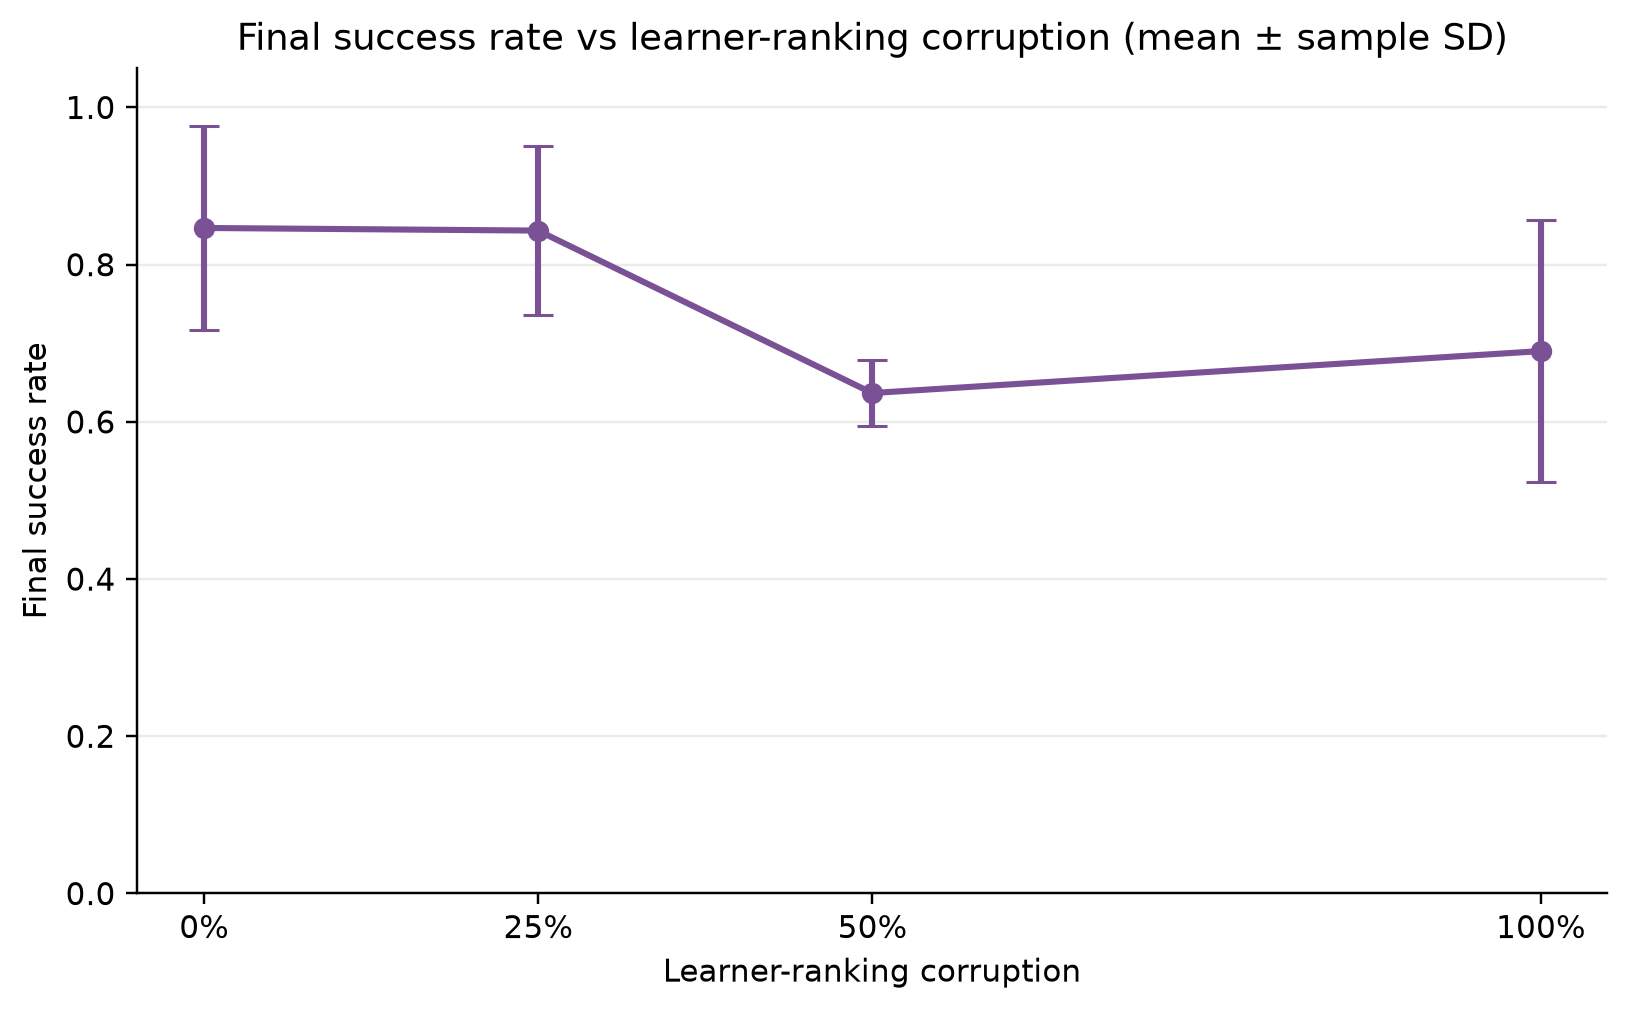
\includegraphics[width=.58\linewidth]{figures/pnp_ranking_robustness.png}
  \caption{Reverse Learner development success under one pre-frozen ranking
  realization per level; 100\% is a fully random permutation. Error bars are
  sample SD across three matched training seeds.}
  \label{fig:robustness}
\end{figure}

The 25\% condition is essentially unchanged, while 50\% corruption degrades
final and hard-group success. A fully random ranking partially recovers. This
may reflect interactions among stage composition, optimization, and the finite
trajectory set rather than one scalar notion of ranking quality. A reliable
response curve would require multiple independent corruptions per level and
more training seeds.

A second task provides an exploratory near-floor comparison. On stacking,
Uniform obtains
$8.33\!\pm\!5.75$\% Fresh-ID success, while Reverse Learner obtains
$2.50\!\pm\!2.00$\%; no curriculum exceeds Uniform. Appendix~\ref{app:stacking}
gives the full experiment. Low success, different representations,
precision-phase emphasis, and different physical criteria prevent treating
this as a decisive reversal or attributing it to task identity alone.

\section{Discussion}
\label{sec:discussion}

\paragraph{Difficulty definitions are not interchangeable.}
Task and Expert difficulty are strongly related ($\rho=0.842$) because the
deterministic expert converts longer approach and transport geometry into
longer executions. Learner difficulty instead measures normalized motion error
of a particular fitted MLP family. It correlates negatively with duration
($\rho=-0.542$), and 43 of 80 Learner-Hard trajectories are Task-Easy. Grasp
and release have the largest phasewise errors, but the score is a per-step
average; these facts make trajectory length and manipulation-phase composition
plausible contributors to ranking disagreement, not established causes.

\paragraph{Staged curricula combine ordering and reweighting.}
Forward schedules expose the first group to about 60\% of all sampled
transitions and the last to only 11--12\%, whereas Reverse Learner assigns
60.1\% to Learner-Hard. The comparison therefore does not isolate ordering
from cumulative exposure. The random-ranking control preserves this staged
mechanism but changes membership: its 69.0\% development success lies below
original Reverse Learner (84.7\%) and Uniform (75.7\%). One corruption per
level, a non-monotonic response, and three seeds prevent interpreting this as
a clean causal effect of ranking quality.

\paragraph{Reverse Learner is uncertain and setting-dependent.}
Its pick-and-place Fresh-ID mean is highest (81.5\% versus 69.3\% for
Uniform), but paired seed differences are $+9.5$, $+28.0$, and $-1.0$
percentage points. Development AUCs are nearly equal (0.787 versus 0.784), and
some intermediate Uniform checkpoints perform strongly; the final mean does
not imply faster convergence. In exploratory stacking, every method is near
the floor and no curriculum exceeds Uniform. Stacking also changes
representation and applies precision-phase emphasis to every schedule, so the
cross-task contrast cannot be attributed solely to task identity.

\paragraph{Closed-loop outcomes matter.}
Final validation losses occupy a narrow range while rollout success varies
widely. One-step imitation metrics therefore remain diagnostics rather than
surrogates for physical completion: errors in grasping, alignment, release, or
retreat alter subsequent states. This gap directly addresses RQ2 and motivates
evaluating curriculum schedules through autonomous closed-loop success.

\section{Limitations}
\label{sec:limitations}

\paragraph{Statistical and schedule scope.}
Only three training seeds are available, with large variation for several
methods. We test one three-stage pacing schedule, without Reverse Task or
Reverse Expert. Moreover, staged eligibility changes cumulative sample
exposure as well as order, so these factors are not independently controlled.

\paragraph{Difficulty construction.}
Task and Expert components are manually chosen, and Expert duration, path
length, and cumulative action magnitude are redundant. Target radius enters
Task difficulty but is absent from the policy observation. Learner difficulty
depends on the MLP, its OOF training protocol, per-step averaging, trajectory
length, and phase composition; alternative choices could change the ranking.

\paragraph{Task and model coverage.}
Only pick-and-place and stacking are studied with small state-based MLPs.
Stacking has near-floor success and may not have converged to a useful regime.
It also uses relative features, precision-phase balancing, and stricter
persistent-contact success, preventing clean attribution of cross-task changes
to task identity.

\paragraph{Simulation and demonstration source.}
All demonstrations come from deterministic scripted experts in PyBullet. We
do not test human data, sensor or actuation noise, other policy families, real
robots, or sim-to-real transfer. The conclusions therefore concern this
controlled simulation study.

\section{Conclusion}
\label{sec:conclusion}

This study asks how the definition of demonstration difficulty affects
curriculum behavior cloning for robotic manipulation. We compare Task, Expert,
and out-of-fold Learner difficulty under five sampling strategies while
matching the policy, initialization protocol, optimizer, update budget,
dataset, and evaluation tasks. The metrics induce substantially different
rankings, and the three easy-to-hard schedules do not consistently outperform
Uniform.

Reverse Learner attains the highest observed mean pick-and-place success, but
the result is seed-sensitive and is not accompanied by faster development AUC.
The near-floor stacking study provides no decisive cross-task replication.
Because staged eligibility couples ordering and exposure, the experiments
support a cautious conclusion: difficulty definitions and sampling schedules
must be evaluated with matched baselines and closed-loop outcomes rather than
ranking intuition or offline loss alone.


\bibliographystyle{plainnat}
\bibliography{references}

\clearpage
\appendix
\section*{Appendix}
\suppressfloats[t]
\section{Object Stacking}
\label{app:stacking}

\subsection{Environment and expert}
The extension stacks a dynamic red 5~cm cube on a dynamic blue 5~cm cube with
the same Panda robot. Its 29D observation contains end-effector state, object
poses and velocities, gripper opening, and placement tolerance; actions remain
three Cartesian deltas plus a gripper command. Success requires physical
source--support contact, alignment and vertical separation within tolerance,
upright low-velocity cubes, an open gripper, robot retreat, and 20 consecutive
stable control steps. A deterministic finite-state expert approaches, grasps,
lifts, transports, aligns, lowers, releases, and retreats using real contacts.
It succeeds on 20/20 fixed and 100/100 randomized verification tasks.

Figure~\ref{fig:stacking-simulation-sequence} visualizes these physical stages
within one successful rollout. In the last frame the gripper has retreated and
the environment's persistent success detector is true after 21 stable control
steps.

\begin{center}
\begin{minipage}{\linewidth}
  \centering
  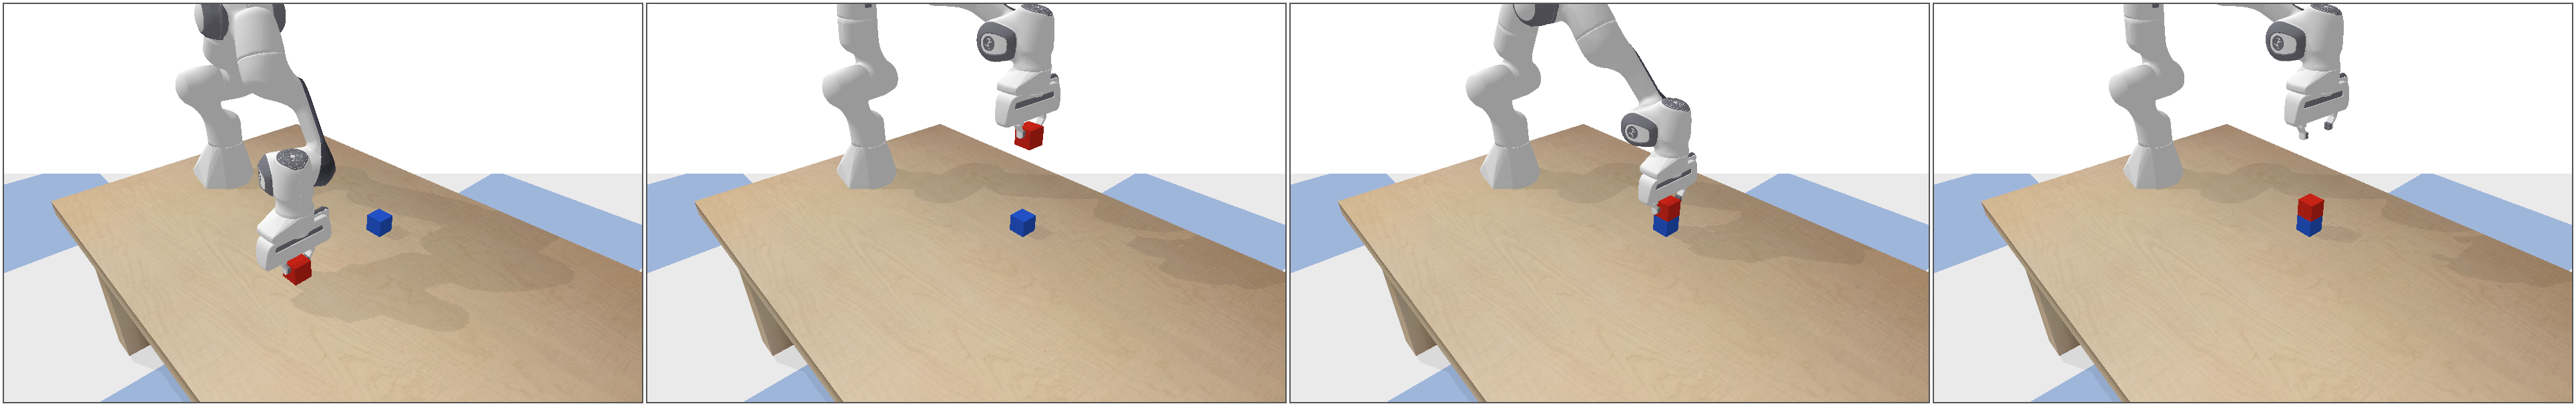
\includegraphics[width=\textwidth]{figures/stacking_simulation_sequence.png}
  \makeatletter
  \def\@captype{figure}
  \makeatother
  \caption{Real PyBullet states from one successful deterministic stacking
  expert rollout: (a) finger grasp of the red source cube, (b) lifted source
  aligned above the dynamic blue support cube, (c) physical source--support
  contact during release, and (d) the stable stack after robot retreat. The
  final frame satisfies \texttt{env.is\_success()} with source--support contact
  and 21 consecutive stable control steps.}
  \label{fig:stacking-simulation-sequence}
\end{minipage}
\end{center}

\subsection{Dataset and behavior cloning}
The frozen dataset contains 300 successful demonstrations and 70,678
transitions, split into 240 training and 60 validation trajectories. Initial
source and support positions vary within conservative reachable ranges, and
placement tolerance is uniform in $[0.012,0.015]$~m. The original scaled BC
obtains 1/100 development successes. Diagnostic analysis identifies large
ALIGN error, phase imbalance, premature release, and closed-loop state shift.
The selected S4.5 representation retains 29 dimensions but replaces source
position with source-minus-end-effector and support position with
source-minus-support. ALIGN, LOWER\_TO\_PRECONTACT, LOWER\_TO\_CONTACT, and
RELEASE transitions receive fivefold effective emphasis. This development
policy obtains 9/100; it is distinct from the matched S6 Uniform models.

\subsection{Difficulty analysis}
Stacking task difficulty replaces object--goal distance with source--support
distance and uses inverse placement tolerance. The Spearman correlations in
Figure~\ref{fig:stack-corr} are $0.802$ (Task--Expert), $-0.102$
(Task--Learner), and $-0.058$ (Expert--Learner). Task and expert scores remain
related, but learner disagreement is weaker than in pick-and-place.

\begin{figure}[!htbp]
  \centering
  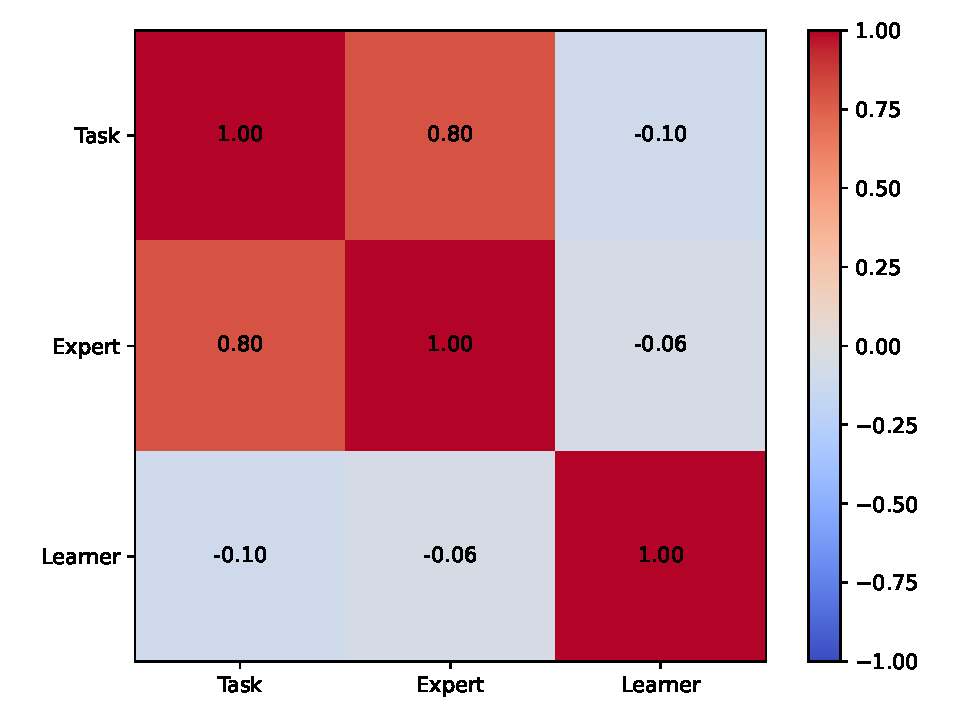
\includegraphics[width=.55\linewidth]{figures/stacking_difficulty_correlation.pdf}
  \caption{Stacking difficulty-score Spearman correlations.}
  \label{fig:stack-corr}
\end{figure}

\subsection{Curriculum results}
All methods use the relative representation and phase emphasis, with emphasis
restricted to the eligible trajectories at each stage. Table~\ref{tab:stack}
reports 200 frozen Fresh-ID tasks (seed 65478). Uniform is strongest, although
all methods are near the performance floor and seed variability remains
material. This exploratory comparison cannot establish a robust reversal of
the pick-and-place ordering.

\begin{table}[!htbp]
\centering
\caption{Stacking final results and development AUC, mean $\pm$ sample SD over
three seeds. Bold marks only the largest observed mean.}
\label{tab:stack}
\small
\begin{tabular}{lcc}
\toprule
Method & Fresh-ID success (\%) & Development AUC \\
\midrule
Uniform & $\mathbf{8.33\!\pm\!5.75}$ & $0.03792$ \\
Task & $3.50\!\pm\!1.32$ & $0.01808$ \\
Expert & $2.50\!\pm\!2.18$ & $0.02667$ \\
Learner & $1.50\!\pm\!1.50$ & $0.01408$ \\
Reverse Learner & $2.50\!\pm\!2.00$ & $0.01175$ \\
\bottomrule
\end{tabular}
\end{table}

\begin{figure}[!htbp]
  \centering
  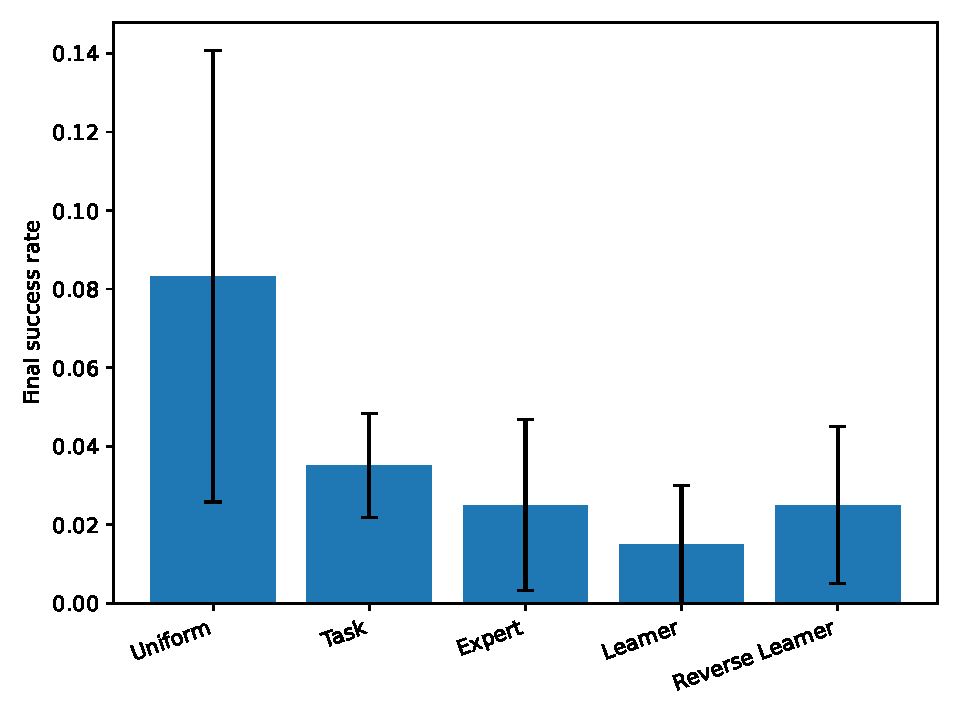
\includegraphics[width=.55\linewidth]{figures/stacking_final_success.pdf}
  \caption{Stacking Fresh-ID success at the predefined 20,600-update
  checkpoint. Error bars show sample standard deviation across three seeds.}
  \label{fig:stack-final}
\end{figure}

\clearpage
\begin{center}
\begin{minipage}{\linewidth}
  \centering
  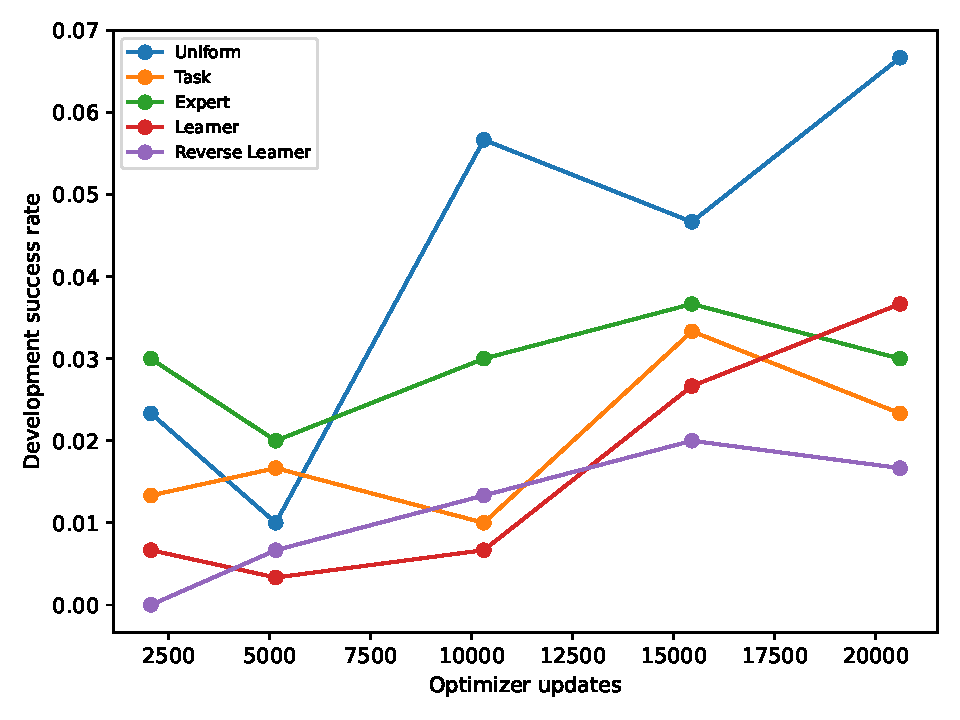
\includegraphics[width=.64\linewidth]{figures/stacking_learning_curves.pdf}
  \makeatletter
  \def\@captype{figure}
  \makeatother
  \caption{Mean stacking development learning curves across three seeds on
  100 frozen tasks; no uncertainty bands are shown.}
  \label{fig:stack-curves}
\end{minipage}
\end{center}

\subsection{Failure analysis}
Failure categories are derived from physical events observed over the rollout.
A grasp/lift failure never raises the source sufficiently; transport/alignment
failure does not move it toward the support; placement/contact failure never
establishes source--support contact; and post-release instability reaches
contact but fails persistent success after opening and retreat. Across all
three seeds, placement/contact dominates (297 failures for Uniform), followed
by post-release instability (195). Reverse Learner has 279 placement/contact
and 245 instability failures. These categories are diagnostic event summaries,
not mutually causal explanations.

\subsection{Cross-task limitations}
Pick-and-place and stacking use 10D and 29D observations respectively.
Stacking additionally uses relative coordinates and phase-balanced training,
and demands persistent contact after release. Overall success is near floor,
so the absence of a curriculum gain is not a strong negative replication.
Only three seeds are available, and the curves do not establish complete
convergence. The cross-task contrast is exploratory and cannot establish that
task identity alone changes the preferred schedule.

\newpage

\section{Additional Results}
\label{app:additional}

\begin{samepage}
\subsection{Hyperparameters}
\begin{center}
\begin{minipage}{\linewidth}
\centering
\makeatletter
\def\@captype{table}
\makeatother
\caption{Shared curriculum-training settings.}
\label{tab:shared-hyperparameters}
\small
\begin{tabular}{ll}
\toprule
Parameter & Value \\
\midrule
Policy & two 128-unit ReLU layers, separate heads \\
Optimizer & AdamW, learning rate $10^{-3}$ \\
Batch size & 256 \\
Updates & 20,600 \\
Checkpoints & 2,060; 5,150; 10,300; 15,450; 20,600 \\
Seeds & 5478, 5479, 5480 \\
Motion objective & scaled MSE \\
Gripper objective & binary cross entropy with logits \\
Early stopping & disabled \\
\bottomrule
\end{tabular}
\end{minipage}
\end{center}
\end{samepage}

The five checkpoints in Table~\ref{tab:shared-hyperparameters} are nonzero;
Figure~\ref{fig:pnp-curves} additionally evaluates the shared update-zero
initialization and includes it in the pick-and-place AUC.

\begin{samepage}
\subsection{Per-seed outcomes}
\begin{center}
\begin{minipage}{\linewidth}
\centering
\makeatletter
\def\@captype{table}
\makeatother
\caption{Stacking Fresh-ID success by training seed (\%).}
\label{tab:stack-seeds}
\small
\begin{tabular}{lrrr}
\toprule
Method & 5478 & 5479 & 5480 \\
\midrule
Uniform & 14.0 & 2.5 & 8.5 \\
Task & 4.5 & 2.0 & 4.0 \\
Expert & 3.5 & 0.0 & 4.0 \\
Learner & 0.0 & 1.5 & 3.0 \\
Reverse Learner & 4.5 & 2.5 & 0.5 \\
\bottomrule
\end{tabular}
\end{minipage}
\end{center}
\end{samepage}

\begin{samepage}
\begin{center}
\begin{minipage}{\linewidth}
\centering
\makeatletter
\def\@captype{table}
\makeatother
\caption{Pick-and-place Fresh-ID success by training seed (\%). The final row
is the seed-matched Reverse Learner minus Uniform difference in percentage
points.}
\label{tab:pnp-seeds}
\small
\begin{tabular}{lrrr}
\toprule
Method & 5478 & 5479 & 5480 \\
\midrule
Uniform & 75.0 & 36.5 & 96.5 \\
Task & 28.0 & 64.5 & 87.0 \\
Expert & 63.5 & 61.5 & 44.5 \\
Learner & 88.0 & 46.5 & 60.0 \\
Reverse Learner & 84.5 & 64.5 & 95.5 \\
Reverse $-$ Uniform & $+9.5$ & $+28.0$ & $-1.0$ \\
\bottomrule
\end{tabular}
\end{minipage}
\end{center}
\end{samepage}

\subsection{Ranking corruption}
For Reverse Learner on pick-and-place, final development success is
$84.7\!\pm\!13.0$\% with the original ranking, $84.3\!\pm\!10.8$\% at 25\%
corruption, $63.7\!\pm\!4.2$\% at 50\%, and $69.0\!\pm\!16.6$\% for a random
ranking. Each nonzero level uses one frozen permutation with the same three
training seeds; 100\% permutes all 240 positions. The non-monotonic pattern is
a sensitivity analysis, not a general law or a complete control for exposure.


\end{document}
